%----------------------------------------------------------------------------------------
%	PACKAGES AND DOCUMENT CONFIGURATIONS
%----------------------------------------------------------------------------------------

\documentclass[a4paper, 12pt]{article}
\usepackage[version=4]{mhchem} % Package for chemical equation typesetting
\usepackage{siunitx} % Provides the \SI{}{} and \si{} command for typesetting SI units
\usepackage{amsmath} % Required for some math elements 
\usepackage{times} % Uncomment to use the Times New Roman font
\usepackage[backend=biber, bibencoding=utf-8, style=chem-acs, citestyle=chem-acs, sorting=none]{biblatex}
\setlength{\parskip}{1em}
\addbibresource{references.bib}
\usepackage{geometry}
\geometry{margin=1in}
\usepackage{textcomp}
\usepackage{graphicx}
\graphicspath{ {./images/} }

%----------------------------------------------------------------------------------------
%	DOCUMENT INFORMATION
%----------------------------------------------------------------------------------------

\title{Separation and Quantitative Analysis of An Unknown Pharmaceutical mixture using RP-HPLC \\ CHEM 4303 \\ Analytical Separations} % Title

\author{Robby \textsc{Renz}} % Author name

\date{\today} % Date for the report

\begin{document}

\maketitle % Insert the title, author and date

\begin{center}
\begin{tabular}{l r}
Date Performed: & October 16, 2018 \\ % Date the experiment was performed
Date Completed: & October 30, 2018 \\
Partner: & Jaya Roe \\ % Partner name
Lab Instructor: & Kevin Stroski % Instructor/supervisor
\end{tabular}
\end{center}

%----------------------------------------------------------------------------------------
%	SECTION 1
%----------------------------------------------------------------------------------------

\begin{abstract}
	High-performance liquid chromatography utilizing the reverse-phase chromatographic technique was used to test the impact of separations by varying the polarity of the mobile phase on a mixture of benzaldehyde, nitrobenzene and chlorobenzene. In addition, this chromatography technique was used to quantitatively identify what was in a unknown pharmaceutical mixture. Finally, it was used to quantitatively analyze one of the unknowns in the mixture with the help of internal standards. For the first part, it was realized that a mobile phase consisting of $70\%$ methanol proved to give a desirable separation for the mixture. In the qualitative part of the experiment, it was concluded that phenacetin and salicylamide were the unknowns in the pharmaceutical mixture.
\end{abstract}
\newpage

%----------------------------------------------------------------------------------------
%	SECTION 2
%----------------------------------------------------------------------------------------

\section{Introduction}
High performance liquid chromatography (HPLC) is a type of chromatographic technique which utilizes high pressure to push the solvent through the column \cite{harris}. In an HPLC, the stationary phase is usually inorganic particles that are made up of silica particles that are microporous \cite{harris}. The type of chromatographic techniques that utilizes this type of stationary phase are normal phase, ion pair, and reversed phase \cite{mold}. Furthermore, one would choose liquid chromatography over gas chromatography for the sole purpose of the analyte in question being not volatile enough to actually undergo gas chromatography \cite{harris}.

In normal phase chromatography, the stationary phase is more polar than the solvent \cite{harris}. However, in reversed phase chromatography, its the exact opposite; the solvent is more polar than the stationary phase \cite{harris}. In reverse phase HPLC, or RP-HPLC, the stationary phase is silica coated with \ce{C18} that acts as a surface \cite{fanali_liquid_2013}. One main advantage of reverse phase over normal phase is that the separation is more reproducible and robust \cite{fanali_liquid_2013}.

In terms of detectors, there are numerous ones that are available for the HPLC. The most commonly used detectors are the ultraviolet-visible detectors and mass spectrometers \cite{vitha_chromatography:_2017}. However, in this experiment, the diode array detector (DAD) is utilized, which is actually a type of UV-visible detector \cite{vitha_chromatography:_2017}. This detector consists of two lamps (tungsten-halogen lamp and a deuterium lamp) that is able to produce electromagnetic radiation, which shine onto a detector array, and its continuously recorded  \cite{vitha_chromatography:_2017}. That way, if its disturbed by the flow of the analyte, the disturbance gets recorded due to the difference in absorption properties \cite{vitha_chromatography:_2017}. This is how it is able to detect analytes.

There are a number of chemicals that are being tested, one of which is acetaminophen, an antipyretic and an analgesic for humans, is known to cause poisons in cats and dogs \cite{dogs-cats}.

There were three main objectives in this experiment; in the first week, the purpose was to test the efficiency of separations in RP-HPLC by varying the composition of the mobile phase (methanol). In the qualitative part of the experiment, the purpose was to identify the types of compounds present in an unknown pharmaceutical mixture. Finally, in the quantitative part of the experiment, the purpose was to find out the mass of one of the drugs present in the aforementioned unknown pharmaceutical mixture.

%----------------------------------------------------------------------------------------
%	SECTION 3
%----------------------------------------------------------------------------------------

\section{Chemicals, Methods and Instrumentation}

\subsection{Chemicals}
Benzaldehyde (Sigma Aldrich, Lot: 41696 PKV), nitrobenzene (Alfa Aesar, Lot: A06V040, 99\%, CAS: 98-95-3), methanol (HPLC grade, Caledon, Lot: 103267, CAS: 108-90-7), salicylamide (Sigma Aldrich, Lot: S51885-279, CAS: 65-45-2), phenacetin (Sigma Aldrich, Lot 78C-0014), acetominophen (Sigma Aldrich, Lot: 32F-0073), caffeine (Sigma Aldrich, Lot: 0316B4), and an unknown pharmaceutical mixture was used in this experiment.

\subsection{Instrumentation}
The separation and analysis of the unknown pharmaceutical mixtures, and the standards, were performed on an Agilent 1100 Series, with a 1260 Infinity degasser (both by Agilent Technologies), fitted with a diode array detector (DAD). The type of column used was a Symmetry\textregistered{} \ce{C18} (particle size of \SI{5}{\mu{}m}, diameter of \SI{4.6}{mm}, and a length of \SI{150}{mm}). The flow rate for each analysis was kept at a constant value of \SI{1}{mL/min}, and the injection volume was \SI{5}{\mu{}L} for each analysis.

\subsection{Methods}
In ``testing the retention behavior in RP-HPLC'' part of the experiment, benzaldehyde, nitrobenzene and chlorobenzene, with volumes of \SI{30}{\mu{}L}, \SI{30}{\mu{}L} and \SI{4}{mL}, respectively, were mixed together. \SI{20}{\mu{}L} of this mixture was diluted with \SI{5}{mL} of HPLC-grade methanol. This diluted mixture was analysed in the HPLC utilizing the RP technique, and the mobile phase was varied until the separations were deemed satisfied. Standards were also prepared for benzaldehyde, nitrobenzene and chlorobenzene. For nitrobenzene, \SI{30}{\mu{}L} of it were diluted with \SI{4.3}{mL} of methanol. And from this mixture, \SI{20}{\mu{}L} were diluted with \SI{5}{mL} of methanol. The same procedure was done for making the benzaldehyde standard. However, for the chlorobenzene standard, \SI{4}{mL} of it were added to \SI{60}{\mu{}L} of methanol, and then \SI{20}{\mu{}L} of this mixture was transferred to \SI{5}{mL} of methanol. The UV detection was set at \SI{254}{nm}.

In the qualitative part of the experiment, \SI{0.0615}{g} of an unknown pharmaceutical mixture was grinded with a mortar and pestle, and dissolved in \SI{25}{mL} of methanol. \SI{500}{\mu{}L} of this mixture was added to \SI{5}{\mu{}L} of water and \SI{5}{\mu{}L} of methanol. This diluted mixture underwent RP-HPLC chromatography with an initial condition of $70:30$ methanol:water. This composition would be varied if necessary in order to get an optimal separation of the mixture. Standards of concentration \SI{2}{mg/mL} were made for salicylamide, phenacetin, caffeine and acetominophen so that the compounds in the mixture can be recognized. Note that these standards were diluted \num{10}-fold before being analyzed. The UV detection was set to \num{245} and \num{275} \si{nm}.

Finally, in the qualitative part of the experiment, a series of calibration solutions was prepared with caffeine acting as the internal standard (IS). \SI{500}{\mu{}L} was the volume of caffeine that was added to each calibration solutions. Salicylamide and phenacetin was found out to be the two compounds in the unknown mixture, and phenacetin was chosen to be quantitatively analyzed. Volumes of \SI{100}{\mu{}L}, \SI{300}{\mu{}L}, \SI{500}{\mu{}L}, \SI{1500}{\mu{}L} and \SI{2500}{\mu{}L} of phenacetin was added to each \SI{10}{mL} of volumetric flask. A constant amount of IS was also added each flask (\SI{500}{\mu{}L}), and it was filled with 50\% methanol till the mark. These solutions was analyzed in the RP-HPLC.

%----------------------------------------------------------------------------------------
%	SECTION 4
%----------------------------------------------------------------------------------------

\section{Results and Discussion}

\subsection{Results}
As stated earlier, in the first week of the experiment, the compositions of the mobile phase, methanol, was being varied with HPLC-grade water in order to notice the differences in separations in RP-HPLC. The corresponding chromatograms are given in the appendix (figures 1 to 4), and tables \ref{tab-cf-benzaldehyde}, \ref{tab-cf-nitrobenzene} and \ref{tab-cf-chlorobenzene} summarizes the aforementioned chromatograms in terms of its capacity factors. In addition, figure \ref{fig-capacity-factors} in the results section illustrates the log of the capacity factors of the three compounds as a function of the polarity of methanol, and table \ref{tab-selectivity} shows how the selectivity factor ($\alpha$) varies with the polarity of methanol. Also, figure \ref{fig-selectivity} in the results section illustrate this graphically.

\begin{table}[h!]
	\centering
	\caption{Data that shows how the capacity factor (k') of benzaldehyde differ with the change in composition in methanol.}
	\begin{tabular}{|c|c|c|}
		\hline
		Methanol/\% & k' of benzaldehyde & log k' \\
		\hline
		90 & 0.218 & -0.662 \\
		\hline
		80 & 0.333 & -0.478 \\
		\hline
		70 & 0.497 & -0.304 \\
		\hline
	\end{tabular}
	\label{tab-cf-benzaldehyde}
\end{table}

\begin{table}[h!]
	\centering
	\caption{Data that shows how the capacity factor (k') of nitrobenzene differ with the change in composition in methanol.}
	\begin{tabular}{|c|c|c|}
		\hline
		Methanol/\% & k' of nitrobenzene & log k' \\
		\hline
		90 & 0.274 & -0.562 \\
		\hline
		80 & 0.459 & -0.338 \\
		\hline
		70 & 0.737 & -0.133 \\
		\hline
	\end{tabular}
	\label{tab-cf-nitrobenzene}
\end{table}

\begin{table}[h!]
	\centering
	\caption{Data that shows how the capacity factor (k') of chlorobenzene differ with the change in composition in methanol.}
	\begin{tabular}{|c|c|c|}
		\hline
		Methanol/\% & k' of chlorobenzene & log k' \\
		\hline
		90 & 0.629 & -0.201 \\
		\hline
		80 & 1.138 & 0.056 \\
		\hline
		70 & 2.026 & 0.307 \\
		\hline
	\end{tabular}
	\label{tab-cf-chlorobenzene}
\end{table}

\begin{figure}[h!]
	\centering
	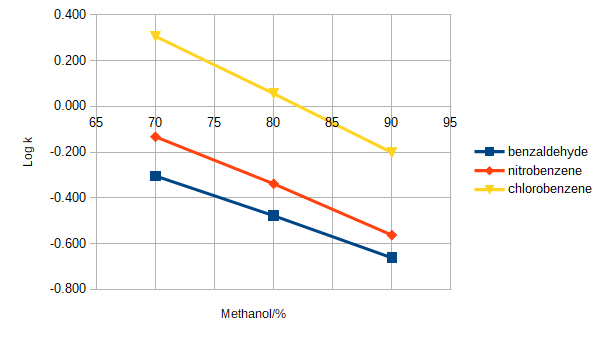
\includegraphics[width=1\textwidth]{fig-capacity-2}
	\caption{Plot of the Log k of benzaldehyde, nitrobenzene and chlorobenzene as a function of the polarity of methanol}
	\label{fig-capacity-factors}
\end{figure}

\begin{table}[h!]
	\centering
	\caption{Data that shows how the selectivity factors ($\alpha$) change with the polarity of methanol.}
	\begin{tabular}{|c|c|c|}
		\hline
		Methanol/\% & Alpha 1,2 & Alpha 2,3 \\
		\hline
		90 & 1.259 & 2.297 \\
		\hline
		80 & 1.377 & 2.478 \\
		\hline
		70 & 1.484 & 2.748 \\
		\hline
	\end{tabular}
	\label{tab-selectivity}
\end{table}

\begin{figure}[h!]
	\centering
	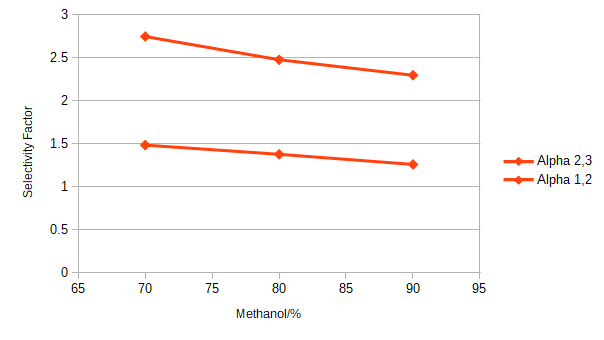
\includegraphics[width=1\textwidth]{fig-selectivity}
	\caption{Plot of the selectivity factors of benzaldehyde, nitrobenzene and chlorobenzene as a function of the polarity of methanol}
	\label{fig-selectivity}
\end{figure}

Figures 5, 6 and 7 show the chromatograms of a chlorobenzene, nitrobenzene and benzaldehyde standards, respectively.

In addition, figure 8 illustrates the chromatogram of the unknown pharmaceutical mixture. While figures 9, 10, 11 and 12 shows the chromatograms of the caffeine, phenacetin, salicylamide and the acetominophen standard, respectively. Note that the optimal composition of the mobile phase was found out to be $50:50$ methanol:water.

Finally, in the quantitative analysis of the experiment, figures 13, 14, 15, 16 and 17 represent the chromatograms \dots{}. Figures 18 and 19 show the chromatograms of the analysis of the aforementioned pharmaceutical unknown. Finally, figures 20, 21 and 22 represents the chromatograms of the blank that was run (50\% methanol).

The pressure of the column for each analysis is shown in table \ref{tab-pressure}. Note that the figure headings correspond to the analysis of the chromatograms in the appendix.

\begin{table}[h!]
	\centering
	\caption{Table that tabulates how the pressure of the column changes with each analysis. The figure number references the chromatogram in the appendix.}
	\begin{tabular}{|c|c|}
		\hline
		Figure number & Pressure/bar\\
		\hline
		Figure 1  & 72 \\ 
		\hline
		Figure 2 & 98 \\
		\hline
		Figure 3 & 122 \\
		\hline
		Figure 4 & 143 \\
		\hline
		Figure 5 & 143 \\
		\hline
		Figure 6 & 143 \\
		\hline
		Figure 7 & 143 \\
		\hline
		Figure 8 & 178 \\
		\hline
		Figure 9 & 178 \\
		\hline
		Figure 10 & 178 \\
		\hline
		Figure 11 & 178 \\
		\hline
		Figure 12 & 178 \\
		\hline
		Figure 13 & 174 \\
		\hline
		Figure 14 & 174 \\
		\hline
		Figure 15 & 174 \\
		\hline
		Figure 16 & 174 \\
		\hline
		Figure 17 & 174 \\
		\hline
		Figure 18 & 174 \\
		\hline
		Figure 19 & 174 \\
		\hline
		Figure 20 & 174 \\
		\hline
		Figure 21 & 174 \\
		\hline
		Figure 22 & 174 \\ 
		\hline
	\end{tabular}
	\label{tab-pressure}
\end{table}

\subsection{Discussion}
The peaks in the chromatogram in figure 4 were able to identified as benzaldehyde, nitrobenzene and chlorobenzene by comparing and matching their retention times to the standards in figures 5, 6 and 7. 

Tables \ref{tab-cf-benzaldehyde}, \ref{tab-cf-nitrobenzene} and \ref{tab-cf-chlorobenzene}, and figure \ref{fig-capacity-factors} clearly show that the capacity factor increases as the percentage of methanol decreases (that is, the polarity of methanol increases). Capacity factor, also known as retention factor \cite{harris}, denotes the time required for the analyte in question to elute \cite{harris}. A greater capacity factor indicates that it is greatly attracted to the column, interacting with the stationary phase \cite{harris}. Therefore, one can conclude that, as it can be clearly seen in figure 4, benzaldehyde is the most polar while chlorobenzene is the least polar of the three compounds; as stated earlier, in RP chromatography, the solvent is more polar than the stationary phase \cite{harris}.

In the quantitative identification of the pharmaceutical unknown mixture, the initial concentration of the mobile phase was chosen as 50\% methanol, and based on the chromatogram received, this composition was considered to be desirable for the analysis of the aforementioned unknown mixture. This was based on the resolution and the retention time for each peaks. Furthermore, by comparing the the chromatogram of the unknown in figure 8 to the standards of the chromatograms in figures 9, 10, 11 and 12, it was realized that the unknown contains the compounds phenacetin and salicylamide. Again, this was determined by cross-referencing the retention times to the standards.

For determining which of the compounds, phenacetin or salicylamide, would be chosen for quantitative analysis, it was agreed that phenacetin would be the ideal option as its peak area is much greater than salicylamide. As for the internal standards, caffeine instead of acetaminophen was chosen as its peak area is similar to phenacetin.

As it can be seen in table \ref{tab-pressure}, the pressure increases whenever the polarity of the mobile phase, in this case methanol, increases (by the addition of water). This is because as one increases the amount of water in the solvent, it increases the viscosity of the solvent, so a higher pressure is required to maintain the flow rate \cite{harris}.

%----------------------------------------------------------------------------------------
%	SECTION 5 (BIBLIOGRAPHY)
%----------------------------------------------------------------------------------------

\section{References}
\printbibliography

%----------------------------------------------------------------------------------------
%	SECTION 6
%----------------------------------------------------------------------------------------

\section{Appendix}

\subsection{Calculations}

\begin{description}
	\item[Calculating the response factor] \hfill \\
		\begin{equation} \label{response-factor}
		\begin{split}
			\frac{\textit{Area of Analyte Signal}}{\textit{Concentration of Analyte}} & = F\Bigg(\frac{\textit{Area of Standard Signal}}{\textit{Concentration of Standard}}\Bigg) \\
			\frac{A_X}{[X]} & = F\Bigg(\frac{A_S}{[S]}\Bigg)
		\end{split}
		\end{equation}
			Equation \ref{response-factor} was taken from \cite{harris}, where $[X]$ and $[S]$ represent the concentrations of analyte and of the standard, respectively.

	\item[$\%$RSD] \hfill \\

	\item[Calculating the capacity factor of chlorobenzene for figure 2 of the chromatogram] \hfill \\
		\begin{equation} \label{equ-capacity-factor}
			\begin{split}
				K & = \frac{t_r - t_m}{t_m} \\
				K & = \frac{2.343 - 1.438}{1.438} \\
				K & = \frac{0.905}{1.438} \\
				K & = 0.629346 \approx 0.629
			\end{split}
		\end{equation}
		Equation \ref{equ-capacity-factor} was taken from \cite{harris}.
\end{description}

\subsection{Chromatograms}
There are 22 sheets of HPLC chromatograms.

%----------------------------------------------------------------------------------------


\end{document}
